\chapter{Architektur}\label{ch-architektur}

Architektureller Aufbau der Softwaresysteme.

\section{Zielarchitektur}

Wie in Kapitel \ref{sec-zielarchitektur} schon beschrieben wurde, ist die
Zielarchitektur für die Darstellung des Dokuments verantwortlich, welche
auf Webtechnologie aufbaut und somit von einem Webbrowser gerendert werden
soll.

Da Webtechnologie, insbesondere HTML/CSS, keine Möglichkeiten bietet
Seiten wie z.B. im DIN A4 Format darzustellen ist \emph{die}
Hauptaufgaben eine geeignete \emph{Abstraktion für Seiten} zu entwickeln.
Eine detailierte Beschreibung ist in Kapitel \ref{sec-abstrationSeiten}.

Weiterhin ist wichtig, wie die einzelnen Entitäten, wie Überschriften,
Texte, Bilder etc. erstellt werden können -- dies soll in Kapitel
\ref{sec-templating} geklärt werden.

Eine Übersicht über die Anforderungen ist in Kapitel
\ref{sec-ziel_anforderungen} aufgelistet.

Im Anhang \ref{appendix-zielarchitektur} sind die wichtigsten Teile des
Quellcodes zu diesem JavaScript-Framework griffig zusammengefasst.
Auch ist im Anhang \ref{appendix-ziel_beispiel} in einem kompletten
Beispiel aufgeführt, wie die einzelnen Klassen zu benutzen sind,
damit daraus ein semi-autoamtisches Dokument erstellt werden kann.
Der kompletten Quellcode mit Tests und weiteren Beispielen ist im
Github Repository \url{https://github.com/themerius/ScalTeX-templates}
zu finden.

\subsection{Anforderungen}\label{sec-ziel_anforderungen}

Das kleine JavaScript-Framework wird mit dem
\emph{behavior-driven development} Paradigma entwickelt,
für diesen Zweck kommt das
Jasmine-Framework\footnote{\url{http://pivotal.github.com/jasmine/}}
zum Einsatz. Folgende Spezifikationen gelten:

\begin{itemize}
  \item Util
    \begin{itemize}
      \item should determine the dpi used by the browser
      \item should calculate the browser specific `pixels per mm`
      \item should be a singleton
      \item should be able to transform mm to px
    \end{itemize}
  \item Entity (siehe Kapitel \ref{sec-templating})
    \begin{itemize}
      \item should create an element out of template and json
      \item should be able to append the created element to another
            element with an id
      \item should know it's actual height
      \item should be able to modify or extend the json
    \end{itemize}
  \item Page (siehe Kapitel \ref{sec-abstrationSeiten})
    \begin{itemize}
      \item should know the type and id for every configured append point
      \item should know it's maximum height for every append point
      \item should create a new element out of a page template and
            configured append points
      \item should be append-able to another element with an id
      \item should know the available space on the page resp. it's
            append points
    \end{itemize}
  \item PageFactory (siehe Kapitel \ref{sec-abstrationSeiten})
    \begin{itemize}
      \item should save the (maybe incomplete) page configurations
            with a related name
      \item should combine the page configs with other page config fragments
            to a complete page config
      \item should produce Page instances out of a certain page config and
            other page config fragments
    \end{itemize}
  \item Areal (siehe Kapitel \ref{sec-areal})
    \begin{itemize}
      \item should be able prepare a construction area for every page type
      \item should generate entities out of a json-sequence and keep them
      \item should generate the special entities, which are individual
            for every page
      \item should mount the entities into the targeted construction area
      \item should create new pages for viewing, with footer, and move the
            entities to fill the pages
      \item should keep track of the page numbers of the viewed pages
      \item should be able to destruct the construction areas
    \end{itemize}
\end{itemize}

\subsection{Abstraktion für Seiten}\label{sec-abstrationSeiten}

Um eine solche Abstraktion zu ermöglichen wird die Hilfe von Javascript
benötigt, welches dafür sorgt, an der richtigen Stelle das Dokument auf
seine entsprechenden Seiten umzubrechen.

\paragraph{Vorarbeit}
Zunächst muss mit gewöhnlichem HTML plus CSS eine „Webseite“ angefertigt
werden, die den Inhalt in eine z.B. DIN A4 Seite hüllt. Diese Konstruktion
kann später von dem Javascript-Framework vervielfältigt und mit entsprechendem
Inhalt gefüllt werden. Wie es beispielhaft auf auf Abbildung
\ref{fig-one_page} zu sehen ist,
kann man gut die Seite mit ihren inneren und äußeren
Grenzen erkennen. Wenn jetzt weitere Texte und Bilder
hinzukommen, wächst der Inhalt über die Seite hinaus. Wir brauchen nun
eine Strategie, um dies zu vermeiden und neue Seiten einzufügen, auf denen
der Inhalt fortgesetzt werden kann.

\newpage
\begin{figure}[h!]
  \centering
    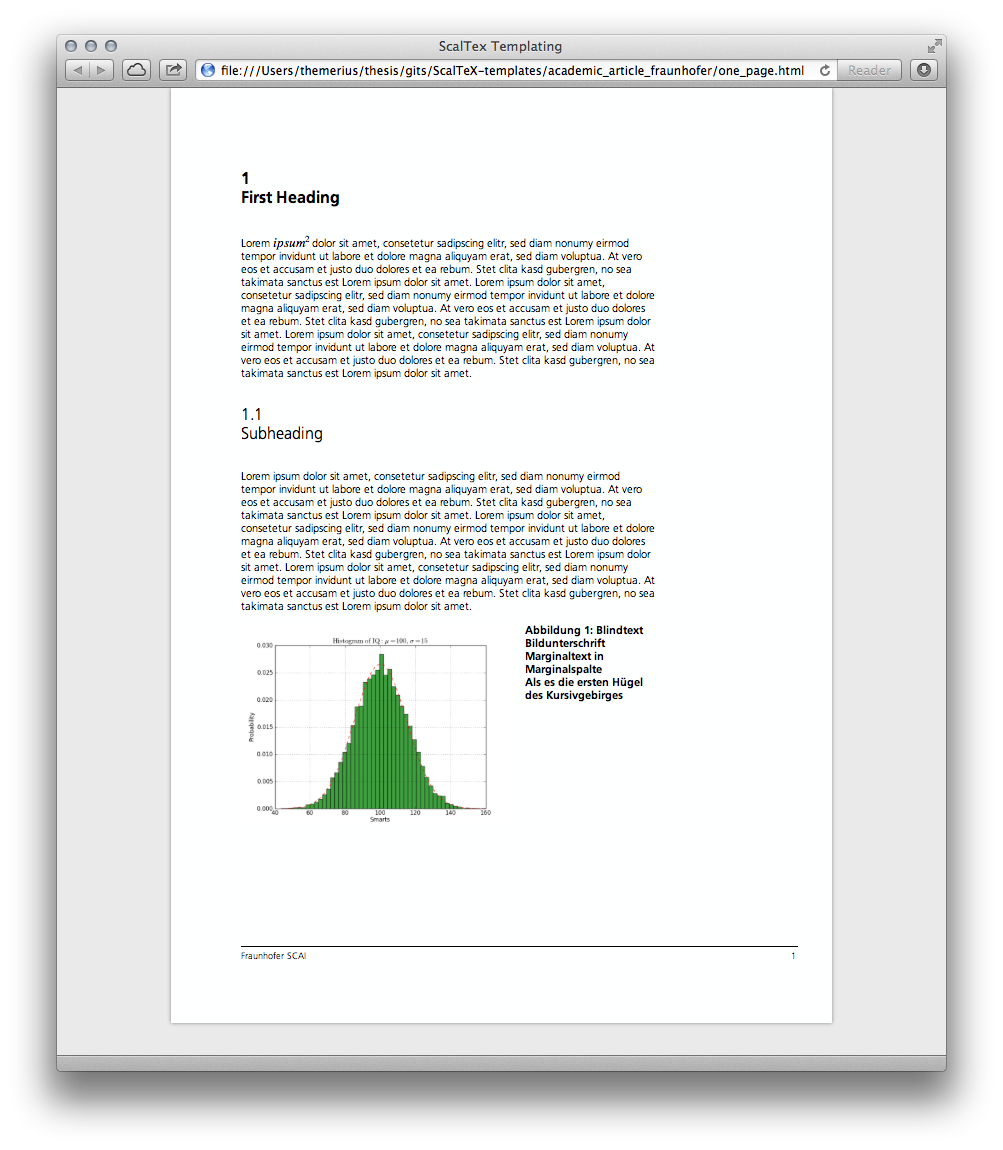
\includegraphics[width=0.9\textwidth]{figures/one_page.png}
  \caption{Einzelne DIN A4 Seite mit HTML und CSS gesetzt.}\label{fig-one_page}
\end{figure}
\newpage

\paragraph{Strategie}
Konzentriert sich zunächst darauf die Entitäten, wie Texte, Bilder usw.,
auf Seiten im Dokumentenfluss zuzuweisen. In diesem Fall darf zunächst eine
einzelne Entität nicht die größe einer Seite überschreiten -- diese
Problematik soll später näher erläutert werden.

Der prinzipielle Ablauf wird auf Abbildung \ref{fig-aufteilungsstrategie}
visualisiert. Rechts ist die temporäre \emph{Construction Page}, die zum
ausmessen der Entitäten dient, für jeden Seitentypus welcher vom jeweilige
Dokumenten-Template geboten wird gibt es also eine Construction Page, sofern
dieser sich von den Ausmaßen anderes verhalten sollte.

Der Ablauf ist also wie folgt: die Entität wird mithilfe der Construction
Page ausgemessen und wenn auf der \emph{View Page} noch genügend Platz
vorhanden ist dort hin verschoben, wenn nicht genügend Platz vorhanden ist,
wir eine neue Seite erstellt und die Entität dort platziert.

Hier kann noch ein Zwischenschritt eingefügt werden, der es ermöglichen
sollte gerade Textentitäten weiter aufteilen zu können, so dass eine
bessere Auslastung der Seiten erreicht werden kann.
% TODO Falls umgesetzt, noch ergänzen.

\newpage
\begin{figure}[h!]
  \centering
    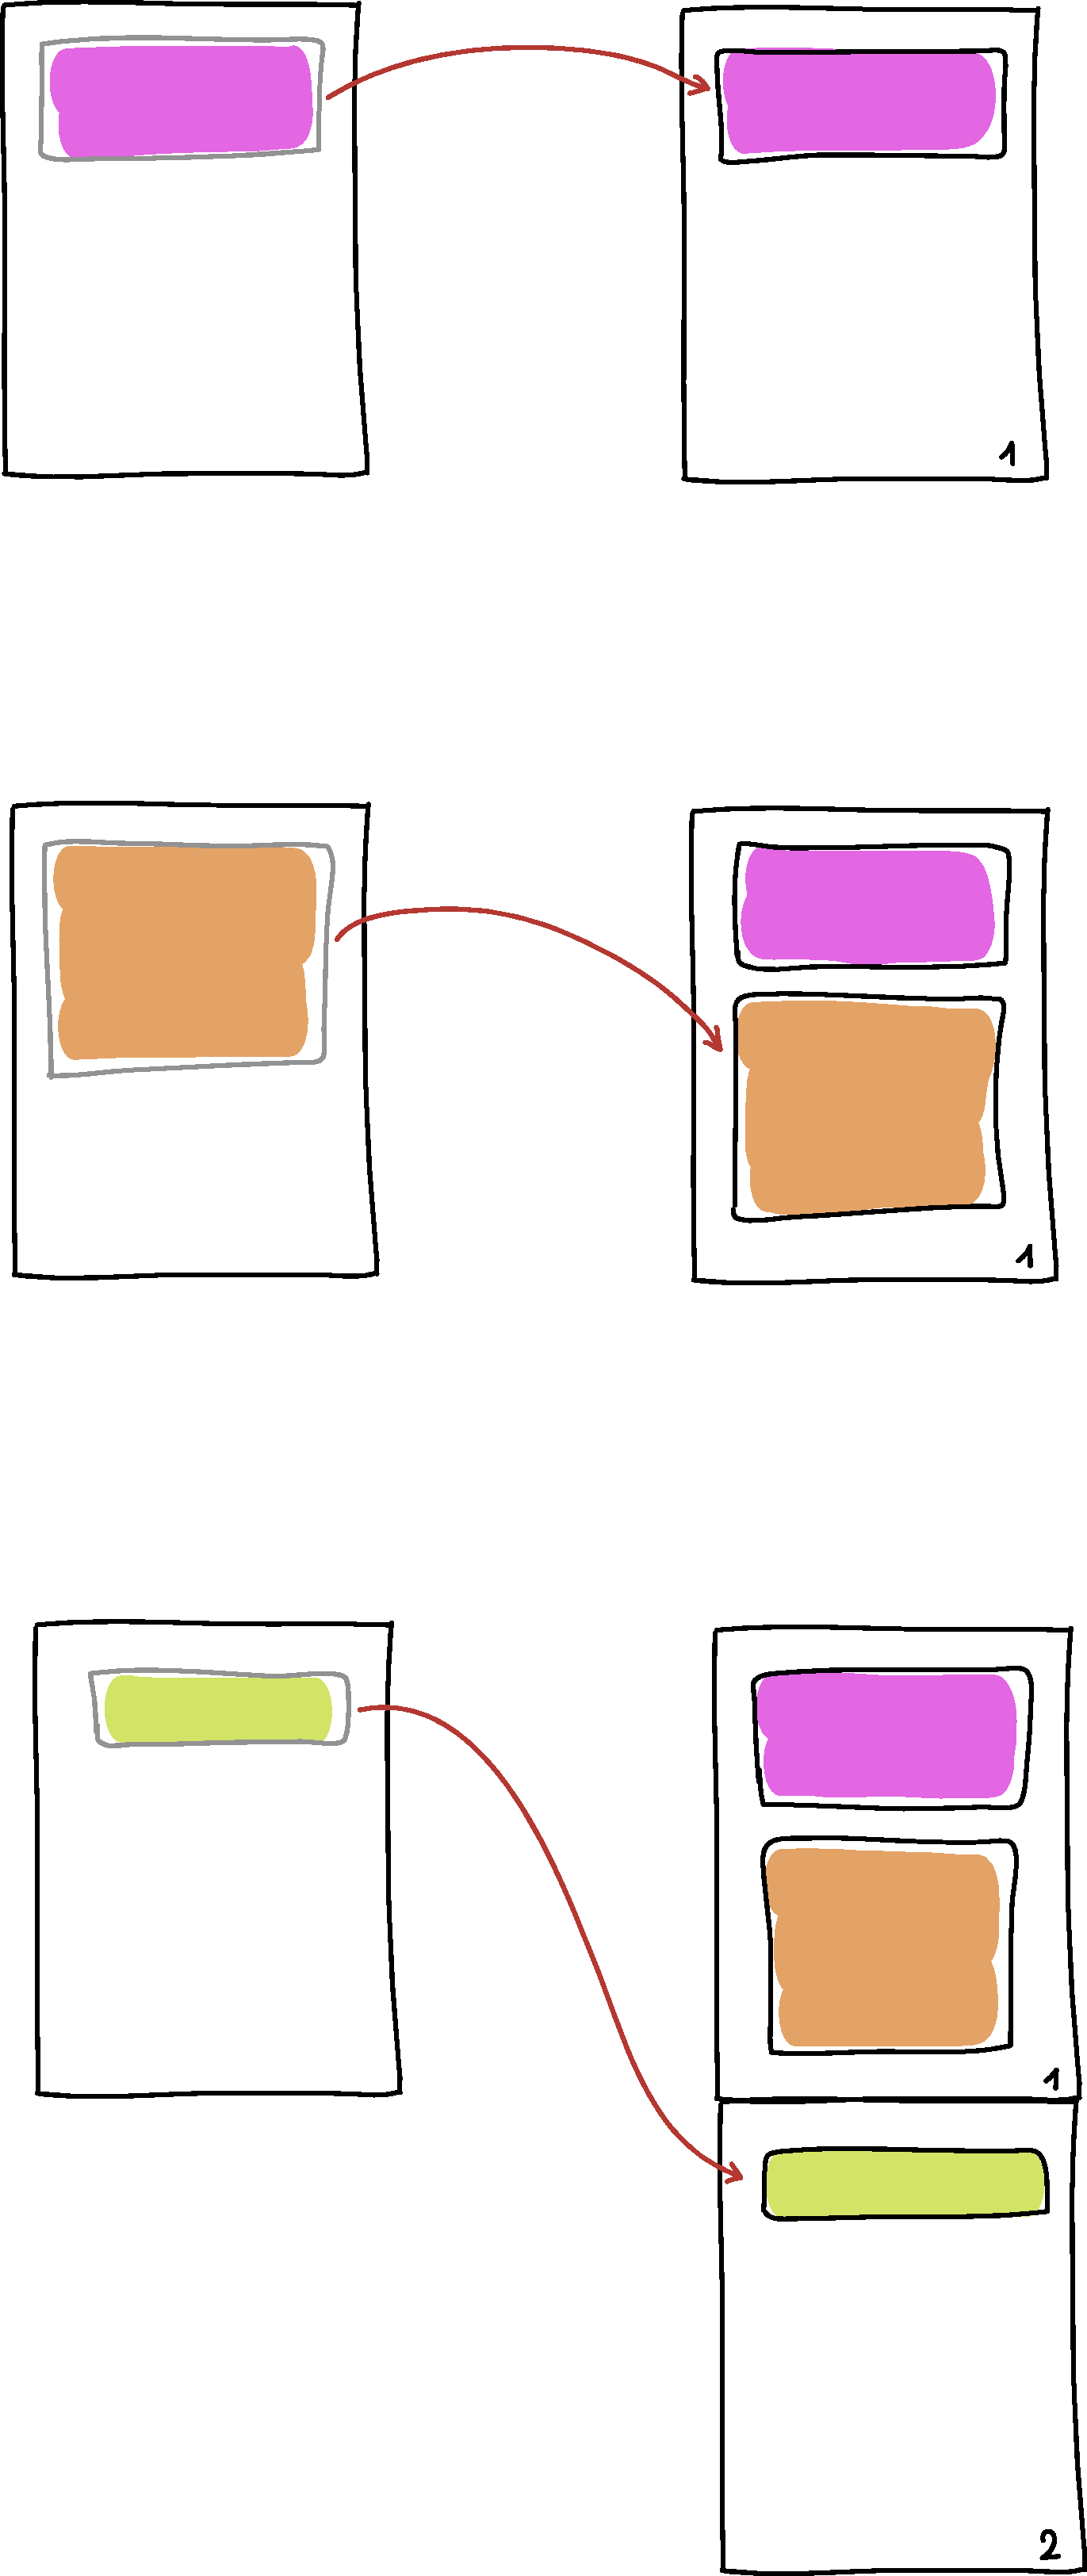
\includegraphics[height=0.9\textheight]{figures/aufteilungsstrategie.pdf}
  \caption{Aufteilungsstrategie, wie Entitäten auf einzelne Seiten
           verteilt werden. Rechts ist die \emph{Construction Page},
           links sind die \emph{View Pages}.}
  \label{fig-aufteilungsstrategie}
\end{figure}
\newpage

\subsection{Templating}\label{sec-templating}

Ich habe mich dazu entschieden das Templating vorerst mit JavaScript
vorzunehmen, also komplett auf der Seite des Dokumenten-Betrachters.
Dies soll den Zweck haben, dass ein Dokumenten-Template-Designer es
leichter haben soll sein Dokumenten-Design zu bauen und zu debuggen --
komplett unabhängig von der DSL bzw. der Programmierlogik.
Zum Einsatz kommt dabei die Javascript-Bib\-lio\-thek
\emph{mustache}\footnote{\url{http://mustache.github.com}}.

Auf diese Weise kann jede einzelne Entität oder Seite clientseitig
durch ein kleines Template-Snippet darstellt werden, welches an die
Bedürfnisse des spezifischen Dokumenten-Designs bzw. Dokumenten-Templates
angepasst ist. Beispielsweise eine Überschrift, könnte so aussiehen.

\begin{verbatim}
<script id="heading" type="text/template">
<div class="row">
  <div class="col4">
    <{{h}}>{{number}}
      </br>
      {{heading}}
    </{{h}}>
    </br></br>
  </div>
  <div class="row-end">&nbsp;</div>
</div>
</script>
\end{verbatim}

Diese muss dann nur noch von der DSL entsprechend mit einer
JSON-Daten\-struktur\footnote{JSON ist die \emph{JavaScript Object Notation},
und bildet die zentrale Datenstruktur von JavaScript.
Mehr Informationen unter \url{http://json.org}.} gefüttert werden.

\subsection{Dokumenten-Areale}\label{sec-areal}

Die resultierenden Seiten zur Anzeige (View Pages), werden bestimmten
Arealen zugeordnet, diese dienen insbesondere der logischen Strukturierung
des Dokuments. Aus Sicht der Seiten sind diese Areale quasi
Einhängepunkte, wo die fertig befüllten Seiten angefügt werden.
Beispiele für Areale sind z.B.

\begin{itemize}
  \item Titelblätter,
  \item Inhaltsverzeichnis,
  \item eigentliches Dokument,
  \item Literaturverzeichnis,
  \item \ldots
\end{itemize}

Innerhalb des HTML-Dokuments können diese Areale in ihrer Reihenfolge
verändert werden, und ermöglichen so einen recht flexiblen Umgang mit
den Doku\-men\-ten-Arealen. Diese sind ganz primitiver HTML-Code wie dieser
z.B.:

\begin{verbatim}
<div id="TitlepageAreal"></div>
<div id="TableOfContentsAreal"></div>
<div id="DocumentAreal"></div>
\end{verbatim}

Es muss nur dem JavaScript-Framework welches die Abstraktion für die
Seiten vornimmt mitgeteilt werden, für welche IDs, welche Areale definiert
sind.


\section{Scala DSL}\label{sec-scalaDSL}

Architektureller Aufbau der auf Scala basierenden internen DSL. Wie in
Kapitel \ref{sec-dsl} beschrieben, wird eine interne DSL in eine bereits
existierende Wirts-Programmiersprache eingebettet und bildet somit
eine mehr oder weniger gewöhn\-liche Software-Bibliothek. Im Idealfall ist
die \emph{API} dieser Bibliothek in ihrer Einsatzdomäne sehr ausdrucksstark.
Wie die API in diesem Fall gestaltet wird, ist in Kapitel \ref{sec-apiDesign}
näher beschrieben.

Scala bietet als Wirtssprache dafür ausgezeichnete Fähigkeiten und
Abstraktionsmittel, wie in Kapitel \ref{sec-grammatikGestaltung} aufgeführt.
Viele dieser Fähigkeiten werden auch bei der Implementierung eingesetzt
und dadruch auch in diesem Kapitel näher beschrieben.

Ein Muster, welches eine wichtige Rolle bei der Erstellung von Dokumenten
spielt, ist der Vorwärtsverweis, also gegenseitige Verweise von Entitäten,
wie Texten, Bildern, etc., aufeinander. Für dieses Muster gibt es in Scala
eine ziemlich elegante Lösung, siehe dazu Kapitel \ref{sec-forwardreference}.

\subsection{Anforderungen}

Kommt noch. Auch behavior-driven development!

\subsection{API Design}\label{sec-apiDesign}

Kommt noch.

\subsection{Bindung zwischen API, Logik und Template}

Kommt noch.

\subsection{Vorwärtsverweis Muster}\label{sec-forwardreference}

Das Problem des
Vorwärtsverweises\footnote{Engl. \emph{forward reference}} tritt auf,
wenn z.B. in einem Text auf eine Abbildung
verweisen wird, welche innerhalb des Programmflusses aber erst später verfügbar
wird.

\begin{lstlisting}
... auf Abbildung {Reference} ist zu sehen ...

Reference = new Figure(...)
\end{lstlisting}

Hier wird also auf \lstinline|Reference| bereits zugegriffen,
bevor sie überhaupt existiert. Erschwerend kommt hinzu, dass sich die
Reihenfolge der Entitäten (Texte, Bilder, etc.) nicht verändert werden darf.
Die Abbilung soll also an der Position im Dokument erscheinen, an der sie
auch im Dokument-Quellcode geschrieben wurde, da es sich hier um eine DSL
handelt, die sich möglichst nahme am eigentlichen Dokument orientiert.

Vollständig beschrieben wird hier die Lösung mit einem \emph{Closure} in
Kapitel \ref{sec-closure}, welches zugleich die eleganteste Lösung darstellt
und auch in der fertigen Implementierung zum Einsatz kommt.

Ein weiterer Ansatz der welcher auch implementiert wurde ist die Lösung
mit \emph{Eval}, welche aber unpraktischer und auch unsicherer einzustufen
ist als die Lösung mit einem Closure. Die in Kapitel \ref{sec-eval}
beschriebene Lösung kommt in der fertigen Implementierung jeodoch nicht
zum Einsatz.

Zudem gibt es noch weitere Überlegungen die während der Lösungsfindung
aufgekommen sind, welche aber nicht weiter verfolgt werden, da die Lösung
mit dem Closure überlegen ist durch höhere Eleganz, Flexibilität und
Sicherheit ist. Daher wird nur kurz auf die anderen Überlegungen in
Kapitel \ref{sec-datenstrukturbasierend} eingegangen.

\subsubsection{Closure}\label{sec-closure}

Insbesondere funktionale Programmiersprachen wie Scala haben die
Möglichkeit Closures zu bilden, d.h. der Teile Geltungsbereich (Scope)
der äußeren Funktion  kann von der inneren Funktion beibehalten werden,
auch wenn der Geltungsbereich der äußeren Funktion bereits verwirkt ist.
% TODO(oder in appendix?)

\begin{lstlisting}
def outer_func = {
  val v = 15
  (x: Int) => x + v  // lambda function
}
\end{lstlisting}

Auf \lstinline|v| kann noch über die Lambda-Funktion zugegriffen werden,
selbst wenn \lstinline|outer_func| nicht mehr exisiert. Teile des
\lstinline|outer_func|-Geltungsbereichts werden quasi mitgezogen.

Genau mit dieser Technik kann man den Vorwärtsverweis in den Griff bekommen.
Es wird der äußere Geltungsbereich eines Objects nach innen gezogen,
um dort später wenn alle Entitäten bekannt sind und die Referenz aufgelöst
wurde darauf zuzugreifen.

\begin{lstlisting}
object O {
  val text = () => s"… auf Abbildung $reference ist zu sehen …"
  val reference = 3
}

O.text()  // wenn reference vorhanden
\end{lstlisting}

Hier wird zudem die Eigenschaft des \lstinline|object| ausgenutzt,
dass die im \lstinline|object| genannten Variablen immer schon vom Compiler
zumindest mit einer \lstinline|null|-Referenz exisieren, aber die Reihenfolge
der eigentlichen Instanziierung wird nicht verändert. Durch das
\lstinline|lazy|-Keyword von Scala, würde die Reihenfolge modifiziert werden
und ist dadurch nicht verwendbar.

Nachteil hier ist, dass der Domänen-Benutzer innerhalb der DSL diese
\lstinline|() => s""|-Magie schreiben müsste -- was zu Verwirrung und
Unverständnis führen würde.


\paragraph{Verbesserung für den Domänen-Benutzer}

Ideal wäre also nun eine Lösung inder der Domänen-Benutzer keine
Aufmerksamkeit auf die Closure-Magie verschwenden muss.

Wie bereits in einem vorherigen Kapitel % TODO(oder in appendix?)
erwähnt wird auf den ab Scala 2.10 verfügbaren
\lstinline|StringContext| (\lstinline|s"…"|) gesetzt.
Dieser lässt sich so erweitern, dass
sich die Closure-Magie verstecken lässt und somit in die API
gezogen wird und der Domänen-Benutzer davon gar nichts mitbekommt.

\begin{lstlisting}
implicit def byname_to_noarg[A](a: => A) = () => a

case class StringContext(parts: String*) {
  def $ (args: (() => Any)*) = () => {
    val unpacked_args = args.map(a => a())
    scala.StringContext(parts: _*).s(unpacked_args: _*)
  }
}

object O {
  val text = $"… auf Abbildung $reference ist zu sehen …"
  val reference = 3
}

O.text()  // wenn reference vorhanden
\end{lstlisting}

\lstinline|byname_to_noarg| ist eine implizite Konvertierung von einem
beliebigen Typ \lstinline|A| mit Call-by-Name
% TODO(fußzeile, appendix "benutzte scala technologien"?)
\lstinline|a: => A| in eine Lambda-Funktion \lstinline|() => a|.

\lstinline|def $| fügt die Möglichkeit hinzu \lstinline|$"…"| als individuell angepassten \lstinline|StringContext| zu verwenden. Es wird eine variable 
Argumentenliste mit den implizit zu Call-by-Name konvertierten Argumenten
aus einem beliebigen \lstinline|$"…"|-String übergeben und in ein Closure gepackt,
welches erst dann ausgeführt wird, wenn die Referenzen auch tatsächlich
vorhanden sind.

% ---> ermöglicht es, in einem Rutsch die Referenzen aufzulösen,
% anders als TeX, welches Zwischenkontexte erstellen muss.

% http://stackoverflow.com/questions/13307418/scala-variable-argument-list-with-call-by-name-possible

% http://stackoverflow.com/questions/13270906/cast-scala-string-to-stringcontext-and-virtually-forward-references

\subsubsection{Eval}\label{sec-eval}

\subsubsection{Datenstrukturbasierend}\label{sec-datenstrukturbasierend}

\paragraph{Request-Queue}

Nur Idee!

\paragraph{Pattern-Matching}

Nur Idee!

\paragraph{„place here“}

Praktikabel mit Xtext-Generator. Prototypisierung ausnutzen (C-Header).
